\documentclass[12pt]{article}
\usepackage[margin=1in]{geometry}

% Font and Language (Computer Modern, xelatex)
\usepackage{polyglossia}
\setmainlanguage{greek}
\setotherlanguage{english}
\newfontfamily\greekfont{FreeSerif}
\newfontfamily\greekfonttt{FreeSerif}

% General
\usepackage{graphicx}
\graphicspath{ {./pictures/} }
\usepackage{caption}
\captionsetup{labelsep=none, font={small,it}}
\renewcommand{\thefigure}{}
\usepackage{float}
\usepackage{ragged2e}
\usepackage{fancyhdr}
\usepackage{titlesec}
\usepackage{xcolor}
\usepackage{minted}
\usepackage{hyperref}
\usepackage{listings}
\usepackage[table]{xcolor}
\arrayrulecolor{black}

% Listings configuration with colors and frame
\lstset{
    backgroundcolor=\color{white},
    frame=single,
    framesep=4pt,
    framerule=0.5pt,
    rulecolor=\color{gray!50},
    basicstyle=\ttfamily\small,
    keywordstyle=\color{blue}\bfseries,
    stringstyle=\color{red},
    commentstyle=\color{green!50!black},
    numberstyle=\tiny\color{gray},
    numbers=left,
    numbersep=5pt,
    stepnumber=1,
    showstringspaces=false,
    tabsize=4,
    breaklines=true,
    breakatwhitespace=false,
    language=VHDL
} 
\hypersetup{
    colorlinks=true,
    linkcolor=blue
}

% Layout
\setlength{\parindent}{0pt}
\setlength{\parskip}{0.5em}

% Title
\title{}
\author{}
\date{}


\begin{document}
    \begin{titlepage}
        \begin{center}
            
            \begin{minipage}{0.3\textwidth}
                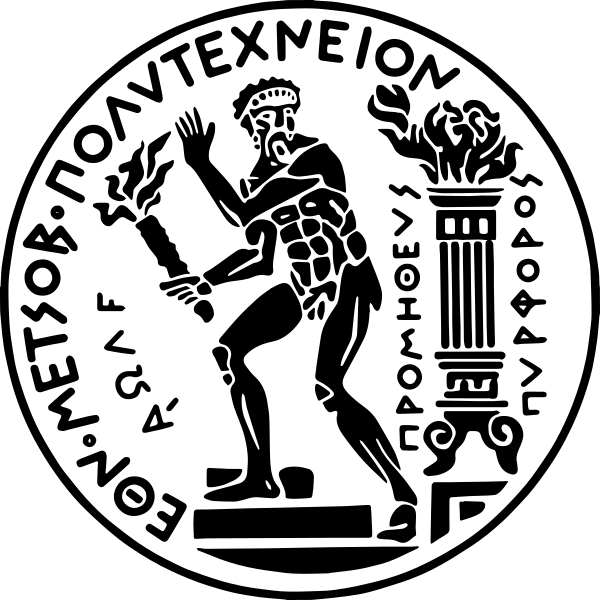
\includegraphics[width=\linewidth]{ntua_logo.png}
            \end{minipage}
            \hfill
            \begin{minipage}{0.65\textwidth}
                \centering
                {\LARGE \textbf{Εθνικό Μετσόβιο Πολυτεχνείο}}\\[0.3cm]
                {\large \textbf{Σχολή Ηλεκτρολόγων Μηχανικών \& Μηχανικών Υπολογιστών}}\\[0.2cm]
                \rule{\linewidth}{0.5pt}\\[0.3cm]
                {\large Εξάμηνο 7\textsuperscript{o}}\\
                {\large \textbf{Ψηφιακά Συστήματα VLSI}}\\
            \end{minipage}
            
            \vspace{2cm}
            
            {\Huge \textbf{1η Εργαστηριακή Άσκηση}}\\[1 cm]
            
            {\Large \textbf{Υλοποίηση Βασικών Ψηφιακών Κυκλωμάτων σε VHDL}}\\[5 cm]
            
            {\Large \textbf{Μέλη Ομάδας}}\\[0.5cm]
            
            \begin{tabular}{rl}
                \textbf{Καβαδάκης Σωτήρης} & 03122035 \\
                \textbf{Κοντοπίδης Δημήτρης} & 03122025 \\
            \end{tabular}
            
            \vfill
            
            {\large Αθήνα, Μάρτιος 2026}
            
        \end{center}
    \end{titlepage}
    \clearpage

% ==============================================================================
% ΜΕΡΟΣ Α
% ==============================================================================
\newpage
\section*{Μέρος Α}
\addcontentsline{toc}{section}{Μέρος Α}

% ------------------------------------------------------------------------------
% Α.2 Decoder 3-to-8
% ------------------------------------------------------------------------------
\section*{Α.2 Decoder 3-to-8}
\addcontentsline{toc}{subsection}{Α.2 Decoder 3-to-8}

\subsection*{Περιγραφή Κυκλώματος}

Ο αποκωδικοποιητής 3-to-8 (Decoder 3 προς 8) είναι ένα συνδυαστικό κύκλωμα που μετατρέπει μια δυαδική είσοδο 3 bits σε μοναδική έξοδο 8 bits. Για κάθε συνδυασμό εισόδου, ακριβώς μία έξοδος είναι ενεργή (λογικό '1'), ενώ οι υπόλοιπες είναι ανενεργές (λογικό '0').

Υλοποιήθηκαν δύο εκδόσεις του κυκλώματος:
\begin{itemize}
    \item \textbf{Behavioral Model}: Χρησιμοποιεί δομή case για περιγραφή της λειτουργίας
    \item \textbf{Dataflow Model}: Χρησιμοποιεί δήλωση with-select για περιγραφή της ροής δεδομένων
\end{itemize}

\subsection*{Σχεδιάγραμμα Λειτουργίας}

\begin{figure}[H]
    \centering
    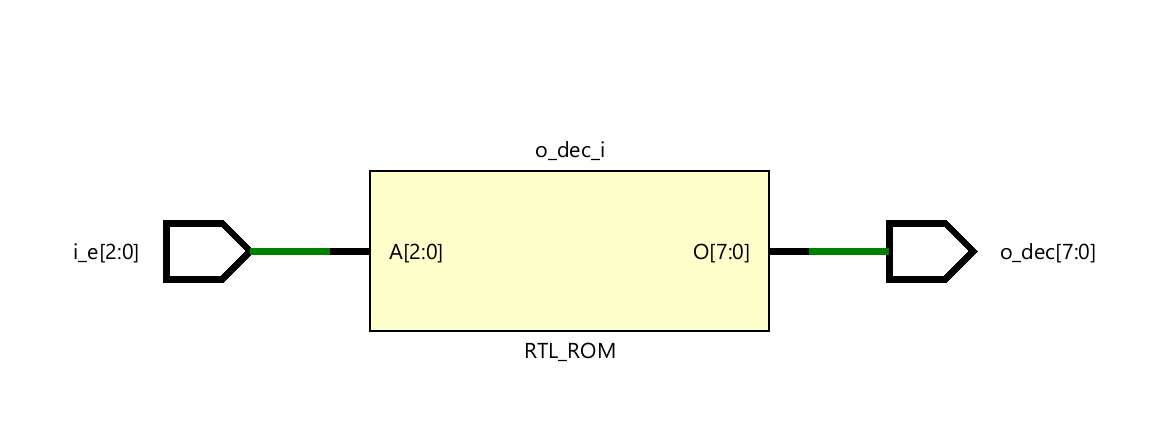
\includegraphics[width=0.7\textwidth]{RTL/decoder.png}
    \caption{RTL σχηματικό του Decoder 3-to-8}
    \label{fig:decoder_rtl}
\end{figure}

Ο πίνακας αλήθειας του Decoder 3-to-8:

\begin{table}[H]
    \centering
    \begin{tabular}{|c|c|}
        \hline
        \textbf{Είσοδος (i\_e)} & \textbf{Έξοδος (o\_dec)} \\
        \hline
        000 & 00000001 \\
        \hline
        001 & 00000010 \\
        \hline
        010 & 00000100 \\
        \hline
        011 & 00001000 \\
        \hline
        100 & 00010000 \\
        \hline
        101 & 00100000 \\
        \hline
        110 & 01000000 \\
        \hline
        111 & 10000000 \\
        \hline
    \end{tabular}
    \caption{Πίνακας αλήθειας Decoder 3-to-8}
    \label{tab:decoder_truth}
\end{table}

\subsection*{Κώδικας VHDL - Behavioral Model}

\begin{lstlisting}[language=VHDL]
-- 3-to-8 Decoder Behavioral Model

library IEEE;
use IEEE.std_logic_1164.all;

entity decoder_3_8_bh is
    port(
    a : in std_logic_vector(2 downto 0);
    y : out std_logic_vector(7 downto 0));
end;

architecture behavioral of decoder_3_8_bh is
begin
    process(a)
    begin
        y <= "00000000";
        case a is
            when "000" => y(0) <= '1';
            when "001" => y(1) <= '1';
            when "010" => y(2) <= '1';
            when "011" => y(3) <= '1';
            when "100" => y(4) <= '1';
            when "101" => y(5) <= '1';
            when "110" => y(6) <= '1';
            when "111" => y(7) <= '1';
            when others => null;
        end case;
    end process;
end behavioral;
\end{lstlisting}

\subsection*{Κώδικας VHDL - Dataflow Model}

\begin{lstlisting}[language=VHDL]
-- 3-to-8 Decoder Dataflow Model

library IEEE;
use IEEE.std_logic_1164.all;

entity decoder_3_8_df is
    port(
    a : in std_logic_vector(2 downto 0);
    y : out std_logic_vector(7 downto 0));
end;

architecture dataflow of decoder_3_8_df is
begin
    with a select
        y <= "00000001" when "000",
             "00000010" when "001",
             "00000100" when "010",
             "00001000" when "011",
             "00010000" when "100",
             "00100000" when "101",
             "01000000" when "110",
             "10000000" when "111",
             "00000000" when others;
end dataflow;
\end{lstlisting}

Παρατηρούμε ότι και οι δύο υλοποιήσεις παράγουν το ίδιο αποτέλεσμα στο RTL σχηματικό, πράγμα που σημαίνει ότι το vivado έχει βελτιστοποιήσει την υλοποίηση του κυκλώματος.

\subsection*{Testbench}

\begin{lstlisting}[language=VHDL]
-- 3-to-8 Decoder Testbench

library IEEE;
use IEEE.std_logic_1164.all;

entity decoder3_8_tb is
end entity;

architecture tb of decoder3_8_tb is
    component decoder_3_8_bh is
        port(a : in std_logic_vector(2 downto 0);
             y : out std_logic_vector(7 downto 0));
    end component;
    
    signal a : std_logic_vector(2 downto 0);
    signal y_bh, y_df : std_logic_vector(7 downto 0);
    
begin
    DUT_BH : entity work.decoder_3_8_bh(behavioral)
        port map(a => a, y => y_bh);
    
    DUT_DF : entity work.decoder_3_8_df(dataflow)
        port map(a => a, y => y_df);
    
    stimulus : process
    begin
        for i in 0 to 7 loop
            a <= std_logic_vector(to_unsigned(i, 3));
            wait for 10 ns;
            assert y_bh = y_df report "Mismatch at input " & integer'image(i) severity error;
            assert y_bh = std_logic_vector(to_unsigned(2**i, 8)) 
                report "Expected output mismatch" severity error;
        end loop;
        wait;
    end process;
end tb;
\end{lstlisting}

\subsection*{Ανάλυση Αποτελεσμάτων Testbench}

Το testbench ελέγχει εξαντλητικά όλους τους 8 δυνατούς συνδυασμούς εισόδου (0 έως 7). Για κάθε είσοδο, επαληθεύει ότι η έξοδος αντιστοιχεί στην αναμενόμενη τιμή σύμφωνα με τον πίνακα αλήθειας χρησιμοποιώντας εντολές assert. Εφόσον δεν υπήρχε κάποιο assert error statement κατά την εκτέλεση της προσομοίωσης, επιβεβαιώθηκε η ορθή λειτουργία και των δύο υλοποιήσεων (Behavioral και Dataflow).

% ------------------------------------------------------------------------------
% Μετρητής 3-bit Up/Down
% ------------------------------------------------------------------------------
\newpage
\section*{Β.2 Μετρητής 3-bit Up/Down}
\addcontentsline{toc}{subsection}{β.2 Μετρητής 3-bit Up/Down}

\subsection*{Περιγραφή Κυκλώματος}

Ο μετρητής 3-bit Up/Down είναι ένα ακολουθιακό κύκλωμα που μπορεί να μετράει είτε προς τα πάνω είτε προς τα κάτω, κάθε φορά αλλάζοντας την τιμή του κατά 1. Υλοποιήθηκαν δύο εκδόσεις:

\begin{itemize}
    \item \textbf{RTL No Limit}: Μετράει κυκλικά από 0 έως 7 (για up) ή 7 έως 0 (για down)
    \item \textbf{RTL Limit}: Μετράει μέχρι ένα καθορισμένο όριο (lim) που ορίζεται από τον χρήστη
\end{itemize}

Είσοδοι:
\begin{itemize}
    \item \texttt{up}: Επιλογή κατεύθυνσης ('1' = up, '0' = down)
    \item \texttt{clk}: Σήμα ρολογιού
    \item \texttt{resetn}: Ασύγχρονη επαναφορά (ενεργή σε '0')
    \item \texttt{count\_en}: Ενεργοποίηση μέτρησης
    \item \texttt{lim}: Όριο μέτρησης (μόνο για την έκδοση με όριο)
\end{itemize}

Έξοδοι:
\begin{itemize}
    \item \texttt{sum}: Τρέχουσα τιμή μετρητή (3 bits)
    \item \texttt{cout}: Σήμα υπερχείλισης/κάτω ροής ('1' όταν φτάνει τα όρια)
\end{itemize}

\subsection*{Σχεδιάγραμμα Λειτουργίας}

\begin{figure}[H]
    \centering
    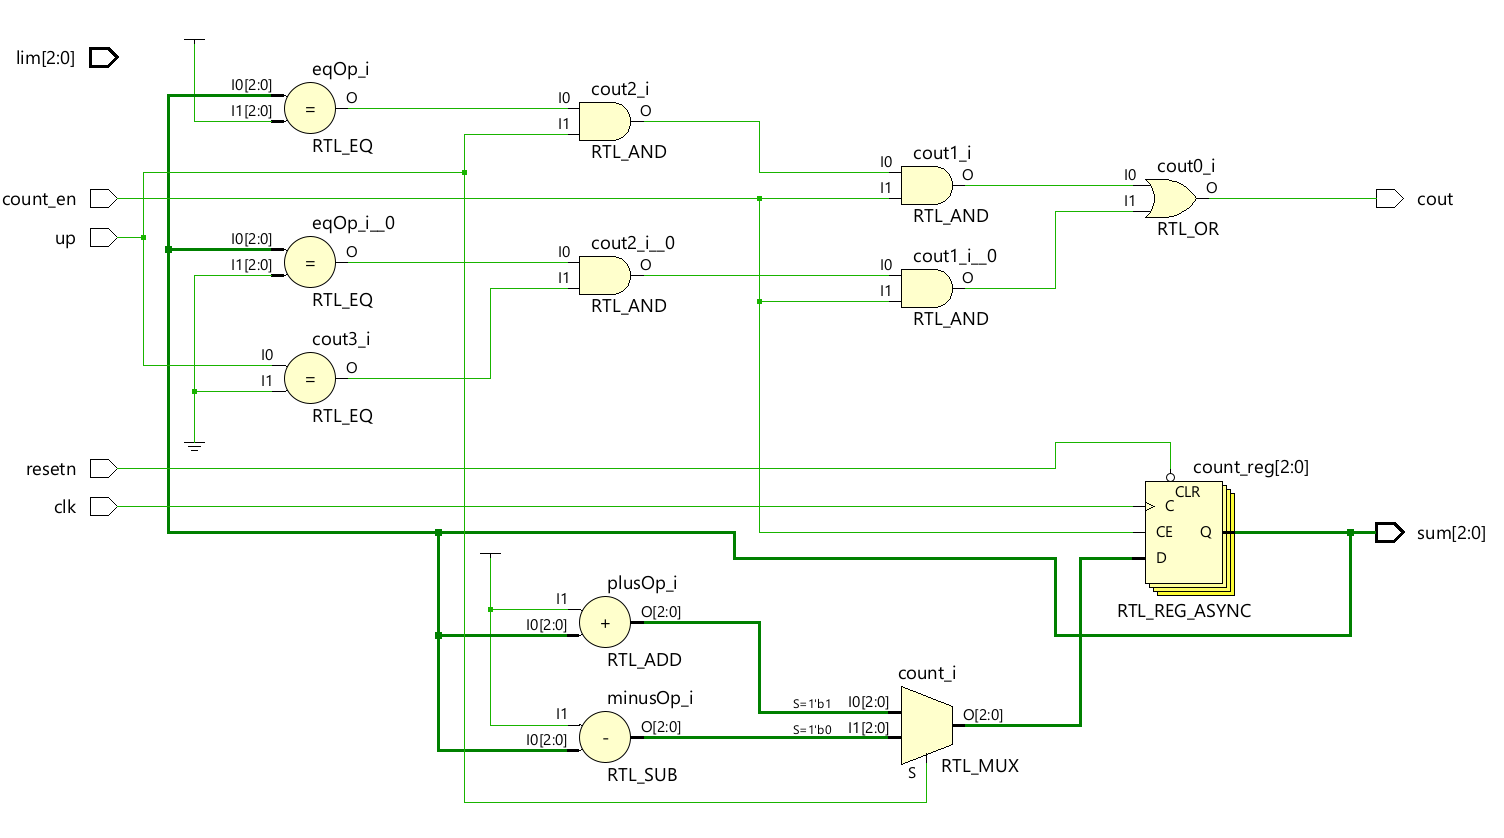
\includegraphics[width=0.9\textwidth]{RTL/counter_nolimit.png}
    \caption{RTL σχηματικό του Μετρητή Up/Down (χωρίς όριο)}
    \label{fig:counter_nolimit_rtl}
\end{figure}

\begin{figure}[H]
    \centering
    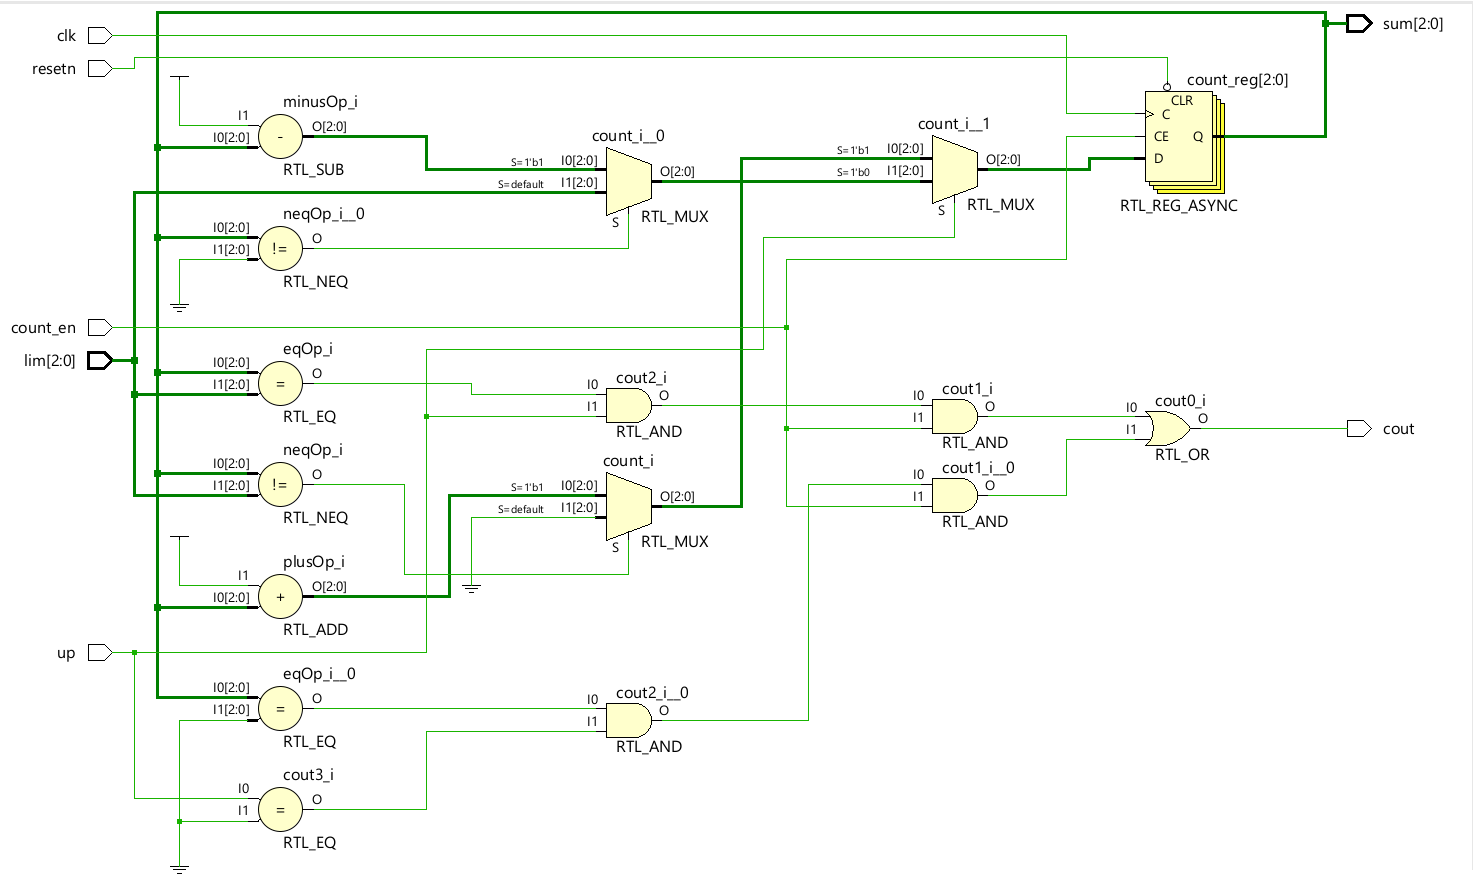
\includegraphics[width=0.9\textwidth]{RTL/counter_limit.png}
    \caption{RTL σχηματικό του Μετρητή Up/Down (με όριο)}
    \label{fig:counter_limit_rtl}
\end{figure}

Η λειτουργία βασίζεται σε 3 flip flops, των οποίων η τιμή μεταβάλλεται στη θετική ακμή του ρολογιού. Συγκεκριμένα, σε κάθε θετική ακμή του ρολογιού, αν η μέτρηση είναι ενεργοποιημένη, η τιμή του μετρητή αυξάνεται ή μειώνεται κατά 1.

\subsection*{Κώδικας VHDL}

\begin{lstlisting}[language=VHDL]
-- 3-bit Up/Down Counter

library IEEE;
use IEEE.std_logic_1164.all;
use IEEE.numeric_std.all;

entity count3_updown is
    port(
        up      : in std_logic;
        clk     : in std_logic;
        resetn  : in std_logic;
        count_en: in std_logic;
        lim     : in std_logic_vector(2 downto 0);
        sum     : out std_logic_vector(2 downto 0);
        cout    : out std_logic
    );
end;

architecture rtl_nolimit of count3_updown is
    signal count : unsigned(2 downto 0);
begin
    process(clk, resetn)
    begin
        if resetn = '0' then
            count <= (others => '0');
        elsif rising_edge(clk) then
            if count_en = '1' then
                if up = '1' then
                    if count = 7 then
                        count <= (others => '0');
                    else
                        count <= count + 1;
                    end if;
                else
                    if count = 0 then
                        count <= to_unsigned(7, 3);
                    else
                        count <= count - 1;
                    end if;
                end if;
            end if;
        end if;
    end process;
    
    sum <= std_logic_vector(count);
    cout <= '1' when (up = '1' and count = 7) or (up = '0' and count = 0) else '0';
end rtl_nolimit;

architecture rtl_limit of count3_updown is
    signal count : unsigned(2 downto 0);
begin
    process(clk, resetn)
    begin
        if resetn = '0' then
            count <= (others => '0');
        elsif rising_edge(clk) then
            if count_en = '1' then
                if up = '1' then
                    if count >= unsigned(lim) then
                        count <= (others => '0');
                    else
                        count <= count + 1;
                    end if;
                else
                    if count = 0 then
                        count <= unsigned(lim);
                    else
                        count <= count - 1;
                    end if;
                end if;
            end if;
        end if;
    end process;
    
    sum <= std_logic_vector(count);
    cout <= '1' when (up = '1' and count = unsigned(lim)) or (up = '0' and count = 0) else '0';
end rtl_limit;
\end{lstlisting}

\subsection*{Testbench}

\begin{lstlisting}[language=VHDL]
-- 3-bit Up/Down Counter Testbench

library IEEE;
use IEEE.std_logic_1164.all;
use IEEE.numeric_std.all;

entity count3_updown_tb is
end entity;

architecture tb of count3_updown_tb is
    component count3_updown is
        port(
            up      : in std_logic;
            clk     : in std_logic;
            resetn  : in std_logic;
            count_en: in std_logic;
            lim     : in std_logic_vector(2 downto 0);
            sum     : out std_logic_vector(2 downto 0);
            cout    : out std_logic
        );
    end component;
    
    signal up      : std_logic := '1';
    signal clk     : std_logic := '0';
    signal resetn  : std_logic := '0';
    signal count_en: std_logic := '0';
    signal lim     : std_logic_vector(2 downto 0) := "101";
    signal sum     : std_logic_vector(2 downto 0);
    signal cout    : std_logic;
    
begin
    clk <= not clk after 5 ns;
    
    DUT_NOLIMIT : entity work.count3_updown(rtl_nolimit)
        port map(up, clk, resetn, count_en, "111", sum, cout);
    
    DUT_LIMIT : entity work.count3_updown(rtl_limit)
        port map(up, clk, resetn, count_en, lim, open, open);
    
    stimulus : process
    begin
        resetn <= '0';
        wait for 20 ns;
        resetn <= '1';
        count_en <= '1';
        
        -- Test count up no limit
        up <= '1';
        wait for 80 ns;
        
        -- Test count down no limit
        up <= '0';
        wait for 80 ns;
        
        -- Test count up with limit
        up <= '1';
        lim <= "101";
        wait for 70 ns;
        
        -- Test count down with limit
        up <= '0';
        wait for 70 ns;
        
        wait;
    end process;
end tb;
\end{lstlisting}

\subsection*{Ανάλυση Αποτελεσμάτων Testbench}

Το testbench ελέγχει και τις δύο αρχιτεκτονικές παράλληλα:

\begin{enumerate}
    \item \textbf{Count Up (No Limit)}: Μετράει από 0 έως 7 και επιστρέφει στο 0 (κυκλικά)
    \item \textbf{Count Up (With Limit)}: Μετράει μέχρι το όριο (π.χ. 5) και επιστρέφει στο 0
    \item \textbf{Count Down (No Limit)}: Μετράει από 7 προς το 0 και επιστρέφει στο 7 (κυκλικά)
    \item \textbf{Count Down (With Limit)}: Μετράει προς τα κάτω μέχρι το 0 και επιστρέφει στο όριο
    \item \textbf{Cout Verification}: Επαλήθευση σήματος υπερχείλισης στα όρια
\end{enumerate}

Η προσομοίωση επιβεβαίωσε την ορθή λειτουργία και των δύο εκδόσεων του μετρητή.

% ------------------------------------------------------------------------------
% Β.3 Shift Register με Parallel Load και Left/Right Shift
% ------------------------------------------------------------------------------
\newpage
\section*{Β.3 Shift Register με Parallel Load και Left/Right Shift}
\addcontentsline{toc}{subsection}{Β.3 Shift Register με Parallel Load και Left/Right Shift}

\subsection*{Περιγραφή Κυκλώματος}

Το κύκλωμα είναι ένα 4-bit shift register με τις ακόλουθες δυνατότητες:
\begin{itemize}
    \item \textbf{Parallel Load (pl)}: Παράλληλη φόρτωση δεδομένων
    \item \textbf{Shift Right (r\_sft='1')}: Ολίσθηση προς τα δεξιά
    \item \textbf{Shift Left (r\_sft='0')}: Ολίσθηση προς τα αριστερά
    \item \textbf{Serial Input (si)}: Σειριακή είσοδος δεδομένων
    \item \textbf{Serial Output (so)}: Σειριακή έξοδος δεδομένων
    \item \textbf{Enable (en)}: Ενεργοποίηση λειτουργίας ολίσθησης
    \item \textbf{Reset (rst)}: Ασύγχρονη επαναφορά
\end{itemize}

\subsection*{Σχεδιάγραμμα Λειτουργίας}

\begin{figure}[H]
    \centering
    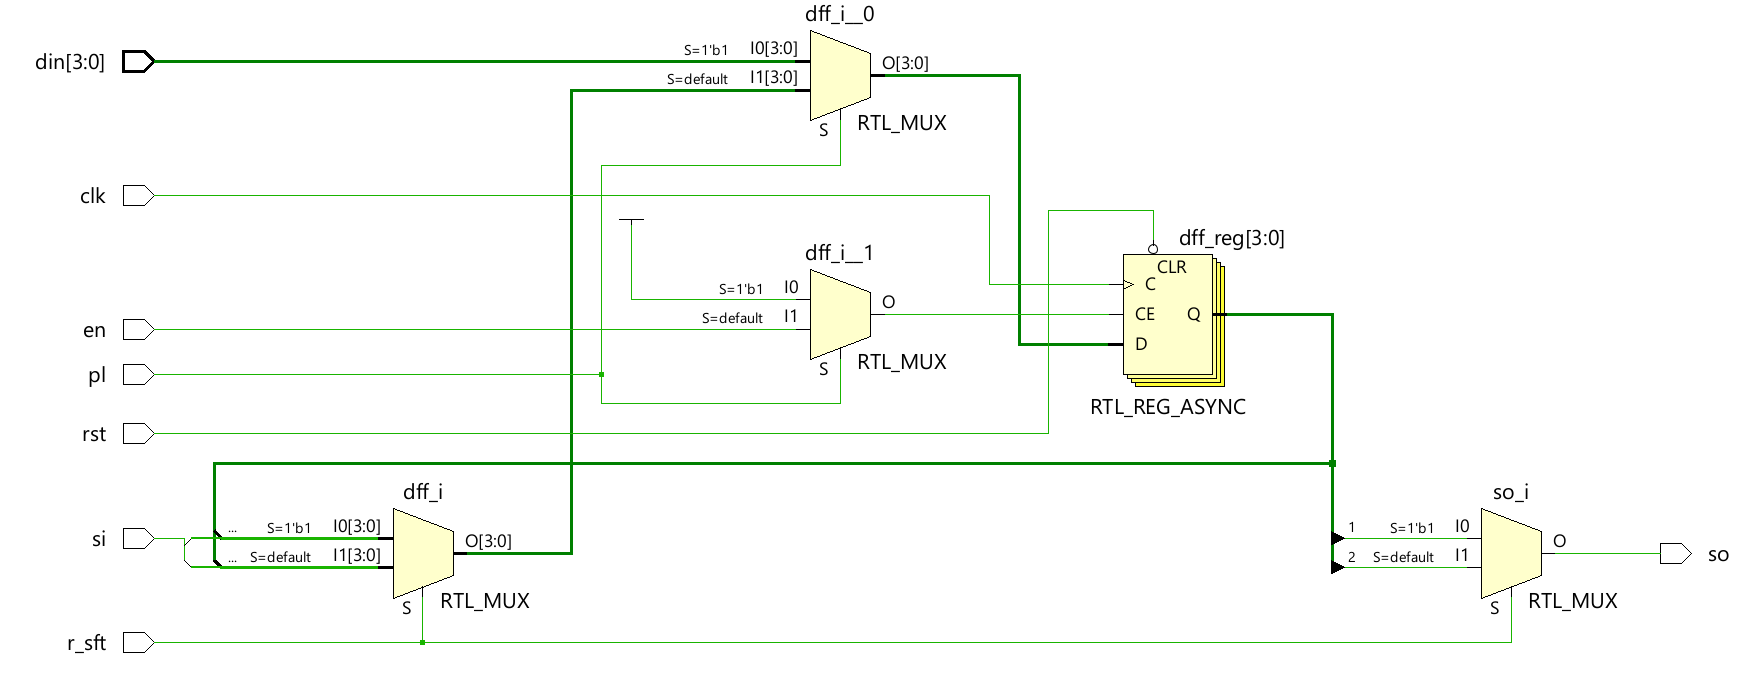
\includegraphics[width=0.9\textwidth]{RTL/shift_register.png}
    \caption{RTL σχηματικό του Shift Register}
    \label{fig:shift_register_rtl}
\end{figure}

Οι είσοδοι ελέγχου λειτουργούν με την ακόλουθη προτεραιότητα:
\begin{enumerate}
    \item \texttt{rst = '0'}: Ασύγχρονη επαναφορά (υψηλότερη προτεραιότητα)
    \item \texttt{pl = '1'}: Παράλληλη φόρτωση δεδομένων από \texttt{din}
    \item \texttt{en = '1'}: Ενεργοποίηση ολίσθησης
    \item \texttt{r\_sft}: Επιλογή κατεύθυνσης ολίσθησης (1=δεξιά, 0=αριστερά)
\end{enumerate}

Η σειριακή έξοδος \texttt{so} εξαρτάται από την κατεύθυνση ολίσθησης:
\begin{itemize}
    \item Shift Right: \texttt{so} = LSB (\texttt{dout(0)})
    \item Shift Left: \texttt{so} = MSB (\texttt{dout(3)})
\end{itemize}

\subsection*{Κώδικας VHDL}

\begin{lstlisting}[language=VHDL]
--------------------------------------------
-- 4 bit shift register with parallel load
--------------------------------------------

library IEEE;
use IEEE.std_logic_1164.all;
entity rl_shift_reg is
    port (
        clk,rst,si,en,pl,r_sft: in std_logic;
        din: in std_logic_vector(3 downto 0);
        dout: out std_logic_vector(3 downto 0);
        so: out std_logic
        );
end rl_shift_reg;

architecture rtl of rl_shift_reg is
    signal dff: std_logic_vector(3 downto 0);
begin
    edge: process (clk,rst)
    begin
        if rst='0' then
            dff<=(others=>'0');
        elsif rising_edge(clk) then
            if pl='1' then
                dff<=din;
            elsif en='1' then
                if r_sft = '1' then
                    dff<=si&dff(3 downto 1);
                else 
                    dff<=dff(2 downto 0)&si;
                end if;
            end if;
        end if;
    end process;
    so <= dff(0) when r_sft = '1' 
                 else dff(3);
    dout <= dff;
end rtl;
\end{lstlisting}

\subsection*{Testbench}

\begin{lstlisting}[language=VHDL]
---------------------------------------------------------------------
-- 4 bit register with parallel load and left/right shift testbench
---------------------------------------------------------------------

library IEEE;
use IEEE.STD_LOGIC_1164.ALL;
use IEEE.NUMERIC_STD.ALL;

entity rl_shift_reg_tb is
end entity;

architecture tb of rl_shift_reg_tb is
    component rl_shift_reg is 
        port (
        clk,rst,si,en,pl,r_sft: in std_logic;
        din: in std_logic_vector(3 downto 0);
        dout: out std_logic_vector(3 downto 0);
        so: out std_logic
        );
    end component;
    
    signal clk : std_logic;
    signal rst : std_logic;
    signal si : std_logic;
    signal en : std_logic;
    signal pl : std_logic;
    signal r_sft : std_logic;
    signal din : std_logic_vector(3 downto 0);
    signal dout : std_logic_vector(3 downto 0);
    signal so : std_logic;
    
    constant CLOCK_PERIOD : time := 10 ns;
    signal expected: std_logic_vector(3 downto 0);
    
begin
    DUT : rl_shift_reg
        port map (
            clk => clk,
            rst => rst,
            si => si,
            en => en,
            pl => pl,
            r_sft => r_sft,
            din => din,
            so => so,
            dout => dout
        );

    STIMULUS : process
    begin
        din <= (others => '0');
        si <= '0';
        en <= '0';
        pl <= '1';
        rst <= '1';
        r_sft <= '0';
        wait until falling_edge(clk);

        -- Test Parallel Load
        for i in 0 to 7 loop 
            din <= std_logic_vector(to_unsigned(i, 4));
            wait until falling_edge(clk);
            assert (din = dout)
                report "PARALLEL LOADING TEST FAILED! Mismatch at input index " & integer'image(i)
                severity error;
        end loop;
        assert false report "PARALLEL LOADING TEST FINISHED!" severity note;

        -- Test Shift Right
        pl <= '1';
        din <= (others => '0');
        wait until falling_edge(clk);

        pl <= '0';
        en <= '1';
        r_sft <= '1';
        si <= '1';
        expected <= (others => '0');
        
        wait for CLOCK_PERIOD * 5;
        assert false report "SHIFT RIGHT TEST FINISHED!" severity note;

        -- Test Shift Left
        pl <= '1';
        din <= (others => '0');
        wait until falling_edge(clk);

        r_sft <= '0';
        si <= '1';
        
        wait for CLOCK_PERIOD * 5;
        assert false report "SHIFT LEFT TEST FINISHED!" severity note;

        wait;
    end process;

    clk_gen : process
    begin
        clk <= '0';
        wait for CLOCK_PERIOD/2;
        clk <= '1';
        wait for CLOCK_PERIOD/2;
    end process;
end tb;
\end{lstlisting}

\subsection*{Ανάλυση Αποτελεσμάτων Testbench}

Το testbench ελέγχει τις ακόλουθες λειτουργίες:

\begin{enumerate}
    \item \textbf{Parallel Load}: Φόρτωση τιμών 0-7 στους καταχωρητές
    \item \textbf{Shift Right με '1'}: Ολίσθηση δεξιά με είσοδο '1' (εμφάνιση σειριακής εξόδου LSB)
    \item \textbf{Shift Right με '0'}: Ολίσθηση δεξιά με είσοδο '0'
    \item \textbf{Shift Left με '1'}: Ολίσθηση αριστερά με είσοδο '1' (εμφάνιση σειριακής εξόδου MSB)
    \item \textbf{Shift Left με '0'}: Ολίσθηση αριστερά με είσοδο '0'
    \item \textbf{Συνδυαστική λειτουργία}: Εναλλαγή μεταξύ parallel load και shift
\end{enumerate}

Η προσομοίωση επιβεβαίωσε την ορθή λειτουργία όλων των λειτουργιών του shift register.

% ==============================================================================
% ΤΕΛΟΣ ΜΕΡΟΥΣ Α
% ==============================================================================

\end{document}